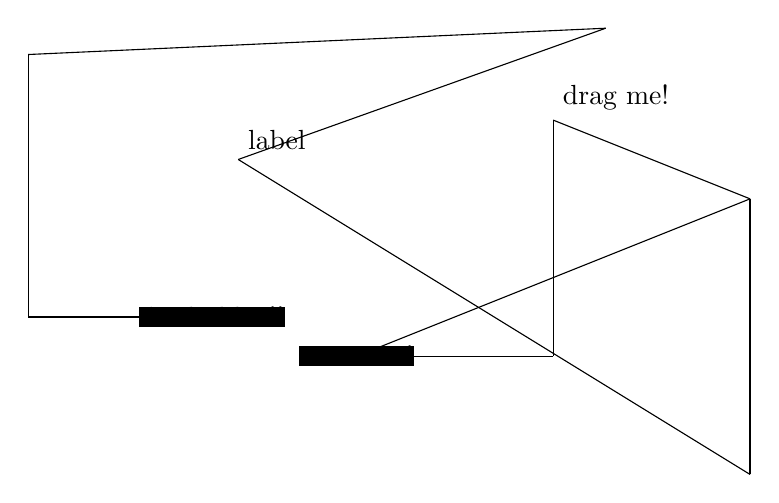
\begin{tikzpicture}[scale=1,
vert/.style={draw,outer sep=0,inner sep=0,minimum size=5,fill},
helper/.style={outer sep=0,inner sep=0,minimum size=5,shape=coordinate},
default_edge/.style={draw},
v2/.style={draw,outer sep=8,inner sep=9,minimum size=10,shape=coordinate,fill=blue,line width=4.2},
every loop/.style={}]

\node (v0) at (6.5,4.5) [vert] {move me!};
\node (v1) at (9,4.5) [v2] {};
\node (v3) at (9,7.5) [v2,label=35:{drag me!}] {};
\node (v5) at (11.5,6.5) [v2] {};
\node (v7) at (11.5,3) [v2] {};
\node (v9) at (5,7) [v2,label=35:{label}] {text};
\node (v11) at (9.667,8.667) [v2] {};
\node (v13) at (2.333,8.333) [helper] {surprise!};
\node (v15) at (2.333,5) [helper] {};
\node (v17) at (4.667,5) [vert] {i'm hidden!!};

\draw[default_edge] (v0) to (v1);
\draw[default_edge] (v1) to (v3);
\draw[default_edge] (v3) to (v5);
\draw[default_edge] (v5) to (v7);
\draw[default_edge] (v7) to (v9);
\draw[default_edge] (v9) to (v11);
\draw[default_edge] (v11) to (v13);
\draw[default_edge] (v13) to (v15);
\draw[default_edge] (v15) to (v17);
\draw[default_edge] (v0) to (v5);
\end{tikzpicture}
